\subsection{Cluster Finding} \label{ssec:framework_cf}
    \begin{wrapfigure}{r}{0.51\textwidth}
        \centering
        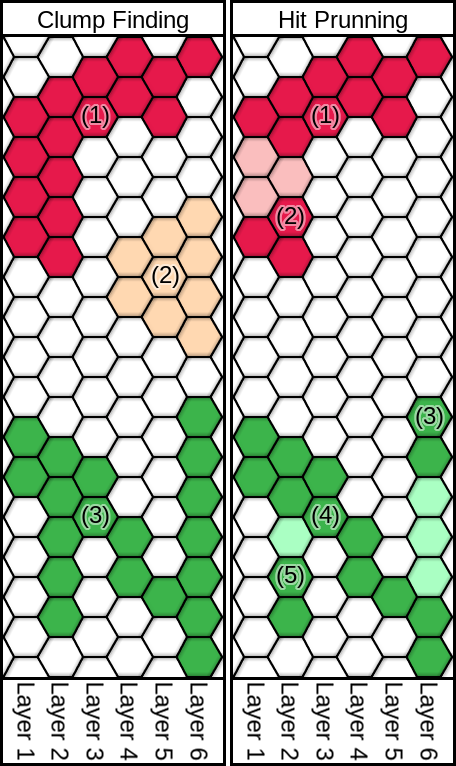
\includegraphics[width=1\textwidth]{clus_finding/00_01}
        \caption{\label{fig:cf_figure1} Clump Finding \& Hit Pruning algorithms over the layers in a superlayer.}
    \end{wrapfigure}

The Cluster Fitting algorithm used at the DC can be described by dividing it into the five algorithms that conform it, which are \textbf{Clump Finding}, \textbf{Hit Pruning}, \textbf{Out of Timers Removal}, \textbf{Cluster Fitting} and \textbf{Cluster Splitting}.

\textbf{Clump Finding}: A clump is defined as a simple set of adjacent hits that spans at least \texttt{DC\_MIN\_NLAYERS} layers, which is a constant at CLAS12 usually set at $4$.
In the image to the left of Figure \ref{fig:cf_figure1}, the clusters formed from a group of hits in one superlayer is denoted.
Each clump formed from the hits is marked using a different color and is also denoted using a simple numbering system.
Running the clump finding algorithm on this group of hits, it can be seen that clumps ($1$) and ($3$) are valid since they span at least $4$ layers while clump ($2$) is invalid for the opposite reason.

\textbf{Hit Pruning}: Hits that are considered noise are pruned in this step.
Four cases are considered for each sequence of hits in a layer: \textbf{(I)} if the sequence contains more than $10$ hits, all hits are considered noise and are removed.
\textbf{(II)} If the sequence contains between $5$ and $10$ hits, only two at each end of the sequence are conserved.
\textbf{(III)} If the sequence contains between $2$ and $4$ hits, only one hit from each end is conserved.
\textbf{(IV)} If $2$ or less hits are in the sequence, no hits are removed.

In the image to the right of Figure \ref{fig:cf_figure1}, the hits removed from each clump are denoted by a lighter color than the ones that stay.
After running the pruning algorithm, the \textbf{Clump Finding} algorithm is ran again on the now pruned hits.
The new clumps are denoted again in the image, with clumps ($2$), ($3$) and ($5$) considered invalid.

\newpage

    \begin{wrapfigure}{l}{0.49\textwidth}
        \centering
        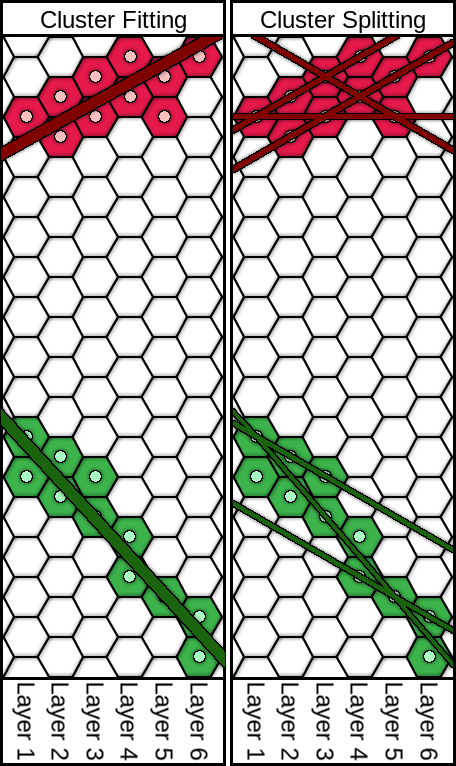
\includegraphics[width=1\textwidth]{clus_finding/02_03}
        \caption{\label{fig:cf_figure2} Cluster Fitting and Splitting algorithms over the layers in a superlayer.}
    \end{wrapfigure}

\textbf{Out of Timers (OOT) Removal}: This method iterates through all the hits in each clump and removes the ones considered Out of Timers.

``Out of Timers'' are hits that have a Distance Of Closest Approach (DOCA) higher than their cell size.
A hit's DOCA refers to the closest distance between the charged particle and the center of the wire in the particle's trajectory, and is measured by analyzing the fluctuations in the wire's charge through time~\cite{blum2008particle}.
A wire's cell size simply refers to the size of the side of the hexagonal cell that contains the wire, as can be seen in Figures \ref{fig:cf_figure1} and \ref{fig:cf_figure2}.

\textbf{Cluster Fitting}: After the clumps are pruned and cleaned from out of timers, a linear fit is attempted for each.
The fit is considered successful if its associated $\chi^2_k$ error is lower than a pre-defined constant threshold named \texttt{HITBASEDTRKGMINFITHI2PROB} (denoted as $\chi^2_{min}$), where $k$, or the number of degrees of freedom, is the number of hits minus $2$.
In the image to the left of Figure \ref{fig:cf_figure2}, a drawing of a possible fit line for each of the clusters obtained in the last step is shown.
$\chi^2$ error is described in Appendix \ref{add:errors}.

\textbf{Cluster Splitting}: When the fitted cluster's $\chi^2_k$ error is above \texttt{MINCHI2}, it becomes necessary to split it and check for better fits using these split clusters.
To do this, all the hits in a cluster are passed through a \textbf{Hough Transform}, which is described in Appendix \ref{add:hough_transform}.
In simple terms, the Hough Transform is a method to detect lines from a set of points via representing these points in a special ``Hough Space''~\cite{duda1971use}.
After the new clusters are formed, only the ones with a $\chi^2_k$ error lower than \texttt{MINCHI2} are accepted.

In the image to the right of Figure \ref{fig:cf_figure2}, multiple lines that could be obtained via the Hough Transform are presented.
It is worth noting that, in the current state of the software, a hit may end up being placed in more than one cluster if these clusters were produced by the Cluster Splitting procedure.